
\section{Apoco Projektstruktur}

Die Abbildung 4.3 veranschaulicht die Paketstruktur der ApoCo-Anwendung.
Sie spiegelt die Modularisierung der ApoCo-Anwendung wieder.
Im Ordner \emph{src} befindet sich der gesamte Quellcode der Anwendung. 
Dieser liegt aufgeteilt in den jeweiligen Modul-Paketen im Hauptpaket der Anwendung \emph{com.janas.apoco}.\\

\subsection*{Paket activity}

Das Paket \emph{activity} beinhaltet alle f\"ur die ApoCo-Anwendung notwendigen Activities.
In diesem Paket befinden sich folgende Klassen:

\begin{itemize}
 \item ActivityBloodpressure:\\
 Hier steht die gesamte Anwendungslogik f\"ur das Protokollieren von Blutdruck.
 Die Activity veranschaulicht in einer scrollbaren Liste alle vorhandenen Messungen.
 Dar\"uber hinaus werden die Daten beim Verlassen der Activity \"uber das Internet mit einem Webserver synchronisiert. 
 
 \item ActivityBodyweight:\\
 Diese Activity behandelt das Protokollieren von K\"orpergewicht des Patienten und beinhaltet die daf\"ur notwendige Anwendungslogik.
 Auch hier werden in einer Listenansicht alle get\"atigten Messungen angezeigt.
 Beim Beenden der Activity werden die Protokolle mit einem Webserver synchronisiert.
 
 \item ActivityDeviceList:\\
 Diese Activity ist notwendig f\"ur das Koppeln \"uber Bluetooth von Sensoren mit dem Smartphone.
 Es ist eine von zwei M\"oglichkeiten des Koppelungsvorgangs in der ApoCo-Anwendung.
 Hier verh\"alt sich das Smartphone wie ein Client.
 Die Activity hat zwei Listen.
 In der einen Liste werden bereits bekannte Ger\"ate aufgelistet.
 Nach einem erfolgreichen Suchvorgang werden die gefundenen Ger\"ate in der zweiten Liste angezeigt.
 Man w\"ahlt aus einen der Listen das gew\"unschte Ger\"at zum Koppeln aus und sie verbinden sich untereinander.
 
 \item ActivityDevices:\\
 Diese Activity bietet die M\"oglichkeit den Koppelungsvorgang zu starten.
 Man w\"ahlt die Art des Messger\"ats aus, zum Beispiel K\"orperwaage, Blutdruckmesser oder Lebensmittelwaage.
 Anschlie\ss{}end w\"ahlt man die Koppelungsart aus.
 Zur Auswahl stehen die M\"oglichkeiten \emph{als Server} und \emph{als Client} zur Verf\"ugung.
 Die Methode \emph{pairing als Client} wird mittels der Klasse ActivityDeviceList ausgef\"uhrt.
 Die Methode \emph{pairing als Server} erledigt die ActivityDevices selbst.
 Daf\"ur startet sie einen Thread mit einem BluetoothServerSocket.
 Dieser h\"ort auf Anfragen von externen Ger\"aten zum Koppeln.

 \item ActivityFoodKcal:\\
 Hier wird der Benutzer drauf aufmerksam gemacht, wieviele Kilokalorien er am aktuellen Tag bereits zu sich genommen hat.
 Zus\"atzlich wird die erlaubte Restmenge berechnet und dem Benutzer angezeigt.
 Wird die erlaubte Tagesdosis \"uberschritten, erscheint eine Warnung auf dem Display.
 In einer Liste werden vorhergehende Mahlzeiten aufgelistet.
 Beim Klicken auf eine Mahlzeit wird die Activity \emph{ActivityMealenergyDetails} als \emph{Dialog} eingeblendet und listet die einzelnen
 Positionen der Mahlzeit mit Informationen \"uber Energie und Gewicht auf.
 Von hier aus gelangt der Benutzer weiter zur Protokollierung einer neuen Mahlzeit und zur Ger\"ate-Koppelung.
 
 \item ActivityMealenergy:\\
 Beim Start ist die Activity immer leer.
 Der Benutzer st\"o\ss{}t von hier aus den Protokollierungsvorgang an.
 \"Uber den Barcode-Button startet der Benutzer eine Activity f\"ur das Scannen von EAN-Codes.
 Anschlie\ss{}end wird eine interne und externe Datenbank nach der gescannten EAN-Nummer durchgesucht.
 Wird ein Eintrag gefunden, so wird der Benutzer zur Activity \emph{ActivityMealContent} weitergeleitet, sonst wird eine Fehlmeldung ausgegeben, dass das Lebensmittel
 nicht identifiziert werden konnte.

 \item ActivityMealenergyContent:\\
 In diese Activity gelangt man nur, wenn das Lebensmittel in der Datenbank identifiziert wurde. 
 Hier werden Detailinformationen \"uber das Lebensmittel angezeigt 
 und \"uber den Button \emph{Waage verbinden?} kann eine Verbindung zur Lebensmittelwaage ge\"offnet werden. 
 
 Nach erfolgreicher W\"agung errechnet die Activity die Energiemenge des gewogenen Lebensmittels, 
 die Gesamtenergie aller Mahlzeiten und
 die noch zur Verf\"ugung stehende Energiemenge f\"ur den aktuellen Tag.

 \item ActivityMealenergyDetails:\\
 Diese Activity erscheint lediglich im Stil eines \emph{Dialog}.
 Das bedeutet, dass die alte Activity im Hintergrund sichtbar bleibt  
 und der modale Dialog tritt wie ein Pop-up in den Vordergrund. 
 Sie besteht nur aus einer scrollbaren Liste und zeigt Details einer Mahlzeit auf.
%  \item ActivityFoodKcalNewEntry:\\

 \item ActivityLogin:\\
 Diese Activity dient dem Anmelden in der ApoCo-Anwendung.
 Alternativ kann ein neuer Benutzer zur Activity \emph{ActivityRegister} wechseln, um sich zu registrieren. 
 
 \item ActivityRegister:\\
 Die Activity tritt als modaler Dialog auf und dient der Erfassung eines neuen Benutzers.
 Hier tr\"agt der Benutzer seine Daten wie Vor- und Nachname, Email und Passwort ein.
 Die Activity f\"uhrt eine Plausibilit\"atskontrolle durch.
 Anschlie\ss{}end sendet sie die Daten an einen Webserver, welcher \"uberpr\"uft, 
 ob der Benutzername bereits vergeben ist. 
 Sollte der Name zur Verf\"ugung stehen, wird der Benutzer in die Datenbank aufgenommen, 
 andernfalls wird er abgelehnt. 
 Die Activity reagiert auf die Serverantwort und akzeptiert entsprechend die Benutzerdaten 
 oder fordert ihn erneut auf seine Eingabe zu \"uberarbeiten.
 
 \item ActivityServerOptions:\\
 Diese Activity erscheint als modaler Dialog und nimmt lediglich die Adresse und Port des Webservers entgegen.
 
 \item ActivitySplashscreen:\\
 Das Splashscreen wird beim Start von ApoCo f\"ur wenige Sekunden angezeigt.
 Diese Activity pr\"asentiert das Logo und den Schriftzug \emph{(Adipositas Controlling}.
 Die Activity beendet sich nach einem Timerablauf automatisch und startet die Start-Activity von ApoCo.

 \item ActivityStart:\\
 Das ist die Hauptactivity in der ApoCo-Anwendung.
 Hier w\"ahlt man die Art der Protokollierung aus.
 Das kann zum Beispiel eine K\"orpergewichtsmessung, Blutdruckmessung oder das Protokollieren der eigenen Nahrungsaufnahme sein.
 Dar\"uber hinaus hat der Benutzer von hier aus den Zugriff auf die Funktion zum Koppeln von Messsensoren.

 %  \item ActivitySummary:\\
\end{itemize}



\begin{figure}[h]
  \centering
  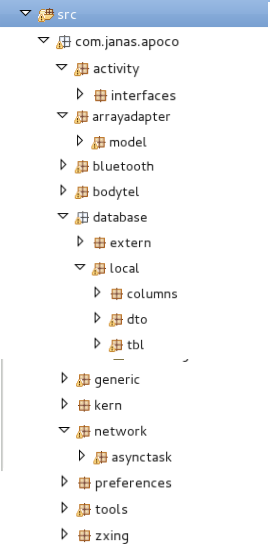
\includegraphics[scale=0.7]{screenshots/kapitel4/projekt_struktur/projekt_struktur_pakete.png}
  \caption{Projekt-Paketstruktur der ApoCo-Anwendung}
  
\end{figure}

\subsection*{Paket interfaces}

Das Paket \emph{activity} beinhaltet au\ss{}erdem das Unterpaket \emph{interfaces}.
Hier befinden sich Java-Schnittstellen, 
welche das Zusammenspiel zwischen Activities und Objekten f\"ur Anwendungslogik unterst\"utzen.
Diese Schnittstellen geben, au\ss{}er einigen Konstanten, auch Objektmethoden vor und werden f\"ur Polymorphie benutzt.
Folgende Interfaces liegen im Paket vor:

\begin{itemize}
 \item AccessableCreatorIF:\\
 Dieses Interface dient zum Erzeugen von unterschiedlichen Threads zur Kommunikation zwischen Software und externen Sensoren.
 F\"ur jeden Sensor steht ein angepasster Thread zur Kommunikation bereit.
 \"Uber dieses Interface wird immer das richtige Objekt durch die jeweilige Activity erzeugt und weitergereicht.

 \item ActivityExtrasCodesIF:\\
 In Android ist es m\"oglich Objekte oder einzelne Werte zwischen den Activities auszutauschen.
 Daf\"ur sind in diesem Interface Konstanten zum Zugriff auf die Daten bereitgestellt, 
 die \"uberall in der ApoCo-Anwendung zwischen den Activities ausgetauscht werden.
 
 \item ActivityRequestCodesIF:\\
 Soll aus einer Activity eine weitere gestartet werden und erwatet man von dieser ein Ergebnis, 
 so wird bei diesem Vorgang ein \emph{RequestCode} mitgegeben.
 Nach Ablauf einer Aufgabe kehrt eine Antwort zur urspr\"unglichen Activity mit dem Ergebnis und \emph{RequestCode} zur\"uck.
 Mit diesem RequestCode kann die Activity unterscheiden welche Antwort sie gerade bekommen hat.
 
 \item CloseableIF:\\
 Eine Activity, die dieses Interface implementiert, darf zum Beispiel von einem Thread oder \emph{Handler} geschlossen werden.
%  \item MessageDisplayableIF:\\
 \item WriteToPerformableIF:\\
 Dieses Interface muss von einer Activity implementiert werden, wenn sie eine Nachricht \"uber Bluetooth versenden muss.
 Die Nachricht wird an ein Thread \"ubergeben und dieser schreibt sie dann in den Streaminput eines \emph{BluetoothSocket}.
\end{itemize}

\subsection*{Paket arrayadapter}

Im Paket \emph{arrayadapter} befinden sich Implementierungen von performanten ArrayAdaptern.
Werden Daten in einer ListView dargestellt,
so kann man sie bequem aus einem Container, 
mittels einem ArrayAdapter in die ListView laden.
Die meisten Listen in ApoCo benutzen keine Standarddarstellung von Daten in einer ListView,
sondern eine individuell zugeschnittene Version.
F\"ur diesen Zweck ben\"otigt man einen zugeschnittenen ArrayAdapter, dessen Funktionalit\"at implementiert werden muss.
Die eigenen ArrayAdapter sind in der Lage Daten zwischenzuspeichern, wenn durch die ListView hin und her gescrollt wird.
Diese Daten m\"ussen nicht mehr nachgeladen werden und das sorgt f\"ur bessere Performance.\\
Im Paket \emph{arrayadapter} befindet sich ein Unterpaket.
Hier werden \emph{Model-Klassen} hinterlegt.
Das sind Daten-Container, welche Informationen f\"ur genau eine Messung speichern.
Zus\"atzlich bietet jedes Model eine statische Methode zum Konvertieren von Datenobjekten in Model-Objekte an. 
Dabei werden die Datenobjekte aus der Datenbank gelesen. 
Jede ListView findet hier einen eigenen ArrayAdapter und das dazugeh\"orige Model.\\

\subsection*{Paket bluetooth}

In diesem Paket befinden sich Klassen und Interfaces, die sich um die Kommunikation \"uber Bluetooth k\"ummern.
\begin{itemize}
 \item AcceptThread:\\
 Diese Klasse ist ein Thread, der einen BluetoothServerSocket startet und auf ankommende Anfragen zur Kommunikation wartet.
 Das ist der erste Schritt von Kommuikationsaufbau.
 
 \item AccessableIF:\\
 \"Uber dieses Interface kommunizieren Activities mit Threads, welche eine BluetoothSocket-Verbindung halten.
 
 \item BluetoothManager:\\
 Der BluetoothManager soll die gesamte Bluetooth-Funktionalit\"at in einer Klasse vereinigen.
 Mit dem BluetoothManager-Objekt wird die Kommunikation aufgebaut, kontrolliert und beendet.
 
 \item ConnectingThread:
 Dieser Thread ist der zweite Schritt zur Kommunikation \"uber Bluetooth.
 Er \"offnet einen Socket zur Gegenstelle und sendet Daten zwischen der Gegenstelle und der Activity.
 
 \item HandlerMessageIF:\\
 Dieses Interface beinhaltet alle Konstanten f\"ur einen Nachrichtenaustausch \"uber einen Handler.
 Die Konstanten erm\"oglichen der Activity zu erkennen, wie sie mit der Nachricht umgehen soll.
 
 \item PairingThread:\\
 Das ist ein Thread, der keine Kommunikation aufbaut.
 Er wird nur ganz kurz f\"ur das Koppeln von Smartphone und einem Sensor genutzt.

 \item StandardUUIDsIF:\\
 Dieses Interface ist vorgesehen, um bekannte standardisierte UUIDs als Konstante bereitzustellen.
 
 \item StartableCanceableIF:\\
 Dieses Interface schreibt einem Thread vor, dass er von Au\ss{}en gestartet und beendet werden kann.
\end{itemize}

\subsection*{Paket bodytel}

Dieses Paket beinhaltet alle Klassen und Interfaces, die notwendig sind, um eine Kommunikation mit Ger\"aten
der Firma Bodytel herzustellen.
Im Augenblick werden die Sensoren WeightTel und PressureTel unterst\"utzt.

\begin{itemize}
 \item BloodpressureResult:\\
 Nach einer Blutdruckmessung wird aus dieser Klasse ein Objekt erzeugt und mit den Messwerten initialisiert.
 Das Objekt wird anschlie\ss{}end in ein Model- und DTO-Objekt konvertiert.
 Das Model-Objekt wird zum Anzeigen in einer ListView genutzt und das DTO-Objekt zum Speichern der Messdaten in der Datenbank.
 
 \item BodyTelUUIDsIF:\\
 Dieses Interface stellt Konstanten bereit, welche von der Firma BodyTel als UUIDs f\"ur die Bluetoothverbindung genutzt werden.
 
 \item BodyweightResult:\\
 Ein Objekt dieser Klasse wird genauso verwendet wie bereits bei der Blutdruckmessung beschrieben wurde, 
 nur dass der Messwert mit der K\"orpergewichtsmessung initialisiert wird.
 
 \item PressureTelConnectedThread:\\
 Dieser Thread baut ein BluetoothSocket zwischen Smartphone und dem PressureTel-Blutdruckmesser auf.
 
 \item PressureTelCreator:\\
 Eine Activity nutzt diese Klasse, um dem BluetoothManager mitzuteilen,
 dass beim Bluetooth-Verbindungsaufbau ein Thread zur Kommunikation mit dem PressureTel gew\"unscht wird.
 
 \item PressureTelMeasurementDecoder:\\
 Diese Klasse dekodiert eine Nachricht von dem Blutdrucksensor.
 Daf\"ur wird die Nachricht in eiem \emph{PressureTelSMS}-Objekt verpackt und alle Messungen,
 die in der Nachricht enthalten sind, als separate \emph{BloodpressureResult}-Objekte
 in einer \emph{List<BloodpressureResult>} zur\"uckgegeben.
 
 \item PressureTelMessageProtocol:\\
 Ger\"ate der Firma BodyTel kommunizieren \"uber eine Art Konversationsprotokoll.
 Um die Messwerte auszulesen, muss dieses Protokoll erf\"ullt werden.
 In diesem Interface werden die notwendigen Konstanten f\"ur die Kommunikation mit dem Sensor \emph{PressureTel} bereitgestellt.
 
 \item PressureTelMessageReader:\\
 Diese Klasse reagiert nach dem Protokoll auf die Anfragen bei der Kommunikation mit dem PressureTel-Blutdrucksensor.
 Sie nutzt die anderen PressureTel-Klassen, um eine Nachricht zu analysieren, auf sie zu antworten, 
 Messwerte aus dieser zu dekodieren und sie in einer Liste an die Activity weiterzugeben. 
 
 \item PresurreTelSMS:\\
 Diese Klasse ist eine Wraper-Klasse f\"ur eine SMS-Nachricht des PressureTel-Sensors.
 Ein Objekt von dieser Klasse wird mit einer SMS initialisiert und konvertiert diese in ein Format,
 dass in ApoCo verwendet werden kann.
 
 \item WeightTelConnectedThread:\\
 Mit diesem Thread wird ein BluetoothSocket zwischen K\"orperwaage und Smartphone ge\"offnet.
 
 \item WeightTelCreator:\\
 Mit Hilfe dieser Klasse erzeugt der BluetoothManager einen Thread, 
 der an die Kommunikation mit der WeightTel-K\"orperwaage angepasst ist.
 
 \item WeightTelMeasurementDecoder:\\
 Diese Klasse wird genutzt, um eine Nachricht der K\"orperwaage zu dekodieren.
 Der Vorgang entspricht dem Dekodierungsvorgang des bereits beschriebenen Dekodierungsvorgangs beim PressureTel-Sensor.
 
 \item WeightTelMessageProtocol:\\
 F\"ur die Kommunikation mit dem WeightTel-Sensor stehen hier die notwendigen Konstanten bereit.
 
 \item WeightTelMessageReader:\\
 Wie beim PressureTel-Sensor, verwaltet diese Klasse den Dekodierungsvorgang einer Messung f\"ur den WeightTel-Sensor.
 
 \item WeightTelSMS:\\
 Diese Klasse ist das zentrale Koppelungselement zwischen einer SMS-Nachricht des WeightTel-Sensors und einer Datenstruktur, 
 die f\"ur ApoCo verwendbar ist.
 
\end{itemize}

\subsection*{Paket Database}

Die Klassen und Schnittstellen in diesem Paket erm\"oglichen einen Zugriff auf die interne und externe Datenbank.
Im Unterpaket \emph{extern} befinden sich zwei Interfaces.
Auf dem Webserver befindet sich in einem bestimmten Verzeichnis die REST-Schnittstelle zum Zugriff auf den MySQL-Datenserver.
Die Schnittstelle \emph{ExternServerDIR} hat eine Konstante, in der das Verzeichnis abgespeichert ist.
F\"ur jede Funktionalit\"at der REST-Schnittstelle gibt es eine entsprechende PHP-Datei.
Im Interface \emph{\texttt{PHP\_URL\_IF}} befinden sich Konstanten mit den Namen der PHP-Dateien.
Zum Beispiel entspricht die Konstante \emph{\texttt{REGISTER\_USER}} der URL \emph{\texttt{register\_user.php}}.
Ruft ApoCo diese URL mit den notwendigen Parametern auf, so ist es m\"oglich einen neuen User im System anzulegen.
Im Unterpaket \emph{local} sind Interfaces und Klasse f\"ur die interne Datenbank auf dem Smartphone.
Das Paket beinhaltet weitere Unterpakete: \emph{column}, \emph{dto} und \emph{tbl}.
Dies geh\"ort zu einem objektorientierten Konzept zum Zugriff auf die Datenbank, welches im Kapitel 4.3 erl\"autert wird.
Des Weiteren enth\"alt das Paket \emph{local} die Klasse DBManagerLocal und das Interface DBManagerPreferencesIF.
Der DBManagerLocal dient jeder Activity als Zugriffsmanager auf die interne Datenbank.
Das Interface DBManagerPreferencesIF dient zum Erstellen und der Konfiguration der Datenbank f\"ur die ApoCo-Anwendung.\\

\subsection*{Paket generic}

In diesem Paket befinden sich drei Klassen f\"ur die Durchf\"uhrung einer W\"agemessung mit der Lebensmittelwaage.
\begin{itemize}
 \item GenericCreator:\\
 Diese Klasse erzeugt einen Thread zur Kommunikation zwischen einer Activity und der KERN PCB-Laborwaage.
 \item KcalConnectedThread:\\
 Dieser Thread baut einen BluetoothSocket mit der Waage auf und kommuniziert mit ihr.
 \item KcalResult:\\
 Diese Klasse repr\"asentiert einen Messwert.
 Er setzt sich aus dem Gewicht und Eigenschaften des gewogenen Lebensmittels zusammen.
 
\end{itemize}

\subsection*{Paket kern}

In diesem Paket ist nur die Klasse \emph{\texttt{KERN\_PCB\_MessageBuilder}} enthalten.
Die Kern-Laborwaage sendet eine Messung als Datenbl\"ocke, die in kurzen Zeitabst\"anden nacheinander empfangen werden.
Diese Datenbl\"ocke werden in der Klasse gesammelt, analysiert und anschlie\ss{}end ein Messwert extrahiert.
Nachdem dieser Vorgang abgeschlossen ist, kann eine Activity \"uber die Methode \emph{readMessage()} den Messwert auslesen.\\

\subsection*{Paket network}

Hier befinden sich alle Klassen und Schnittstellen, die f\"ur eine Kommunikation \"uber WLAN oder das Mobile-Netz 
notwendig sind.
\begin{itemize}
 \item \texttt{JSON\_TAG\_IF}:\\
 Diese Schnittstelle stellt alle \emph{tag}-Namen zur Verf\"ugung, 
 die bei einem Datenaustausch mit dem Webserver im JSON-Format genutzt werden.
 
 \item NetworkHandler:\\
 Diese Klasse ist ein Handler, der in jeder Activity genutzt wird, welche mit dem Webserver kommunizieren muss.
 Vor einem Datenaustausch wird \"uberpr\"uft, ob eine WLAN- oder Mobile-Netz-Verbindung besteht und ob der Webserver antwortet.
 Je nach Ergebnis reagiert der Handler und benachrichtigt den Benutzer, wenn der Server nicht erreichbar ist.
 Eine Activity kann von diesem Handler geschlossen werden.
 Dazu muss sie die Schnittstelle \emph{CloseableIF} implementieren und mit einem Flag best\"atigen.
 Durch die Schnittstelle kann sie beendet werden, aber erst mit dem Flag wird dies auch abh\"angig von der Situation angefordert.
\end{itemize}

Im Unterpaket \emph{asynctask} befinden sich Klassen, welche von der Klasse AsyncTask<T,T,T> abgeleited werden.
Es handelt sich dabei um Threads, die einen Teil der Arbeit im UI-Thread durchf\"uhren und den Hauptteil als Nebenl\"aufigkeit.
Mit diesen Threads wird je eine bestimmte Netzwerkfunktionalit\"at der ApoCo-Anwendung erledigt.\\

\subsection*{Paket preferences}

Dieses Paket beinhaltet den \emph{PreferencesManager} und eine Schnittstelle \emph{\texttt{APOCO\_PREFERENCES}}.
Der \emph{PreferencesManager} behandelt ApoCo-spezifische Parameter.
Normalerweise k\"onnen Werte in einer Datei oder Datenbank persistent gespeichert werden.
Shared Preferences ist eine weitere M\"oglichkeit in Android, 
anwendungsbezogene Werte als eine Art Schl\"ussel-Wert-Paar zu speichern.
Die Schnittstelle \texttt{APOCO\_PREFERENCES} beinhaltet alle Schl\"ussel f\"ur den Zugriff auf die Shared Preferences.\\

\subsection*{Paket tools}

Das Paket \emph{tools} beinhaltet Werkzeuge, die projekt\"ubergreifend n\"utzlich sein k\"onnen.

\begin{itemize}
 \item BloodpressureDiagnose:\\
 Diese Klasse bietet Funktionen, die eine einfache Interpretation von Blutdruckwerten \"ubernehmen.
 Man \"ubergibt Blutdruckwerte an die Methode \emph{performDiagnose()} und bekommt eine Aussage \"uber die Messung.
  
 \item BodyweightDiagnose:\\
 Diese Klasse errechnet die Differenz zwischen Dem Zielk\"orpergewicht und dem aktuellen K\"orpergewicht.
 
 \item ConnectivityTest:\\
 Mit dieser Klasse ist es m\"oglich durch den Aufruf der Methode \emph{isAnyNetworkReachable()} festzustellen,
 ob das Smartphone \"uber WLAN oder Mobile-Netz mit dem Internet verbunden ist.
 
 \item DateTemplateIF:\\
 Diese Schnittstelle enth\"alt verschiedene Datumsmuster als Konstanten f\"ur eine Konvertierung eines Datums in ein 
 gew\"unschtes Format.
 \item FloatPrecision:\\
 Diese Klasse \"uberpr\"uft einen Flie\ss{}kommawert, ob er in der N\"ahe der Zahl 0 liegt. 
 F\"ur den Test ist ein Epsilon f\"ur die Pr\"azision notwendig.
 
 \item HexConverter:\\
 Diese Klasse bietet mehrere Methoden an, um hexadezimal codierte Bytearrays in lesbare Strings umzuwandeln und umgekehrt.
 
 \item JSONParser:\\
 Diese Klasse erleichtert das Senden und Empfangen von JSON-Strings zwischen einer Anwendung und einem Webserver.
 Dabei ist es m\"oglich die HTTP-Methoden POST und GET zu benutzen.
 Die Serverantwort wird als JSON-Objekt zur\"uckgegeben.
 
 \item PasswordCheck:\\
 Diese Klasse \"uberpr\"uft, ob ein Passwort der gew\"unschten Vorgabe entspricht.
 Es wird die Mindestl\"ange und die wiederholte Eingabe des Passwortes gepr\"uft.
 
 \item ResourcesTools:\\
 Diese Klasse ist ein Wraper, um aus Android-Ressourcen eine String-Ressource zu lesen.
 
 \item TimeTools:\\
 Diese Klasse konvertiert einen Timestamp vom Typ Long in einen String mit dem Format \emph{dd-MM-yyyy HH:mm} und umgekehrt.
 
 \item Toasting:\\
 Diese Klasse erleichtert Informationen \"uber einen Toast anzuzeigen.
 Der hier ausgegebene Toast entspricht nicht den Standardvorgaben, sondern ist individualisiert.
 
 \item URLBuilder:\\
 Diese Klasse bietet die Methode \emph{getURL()} an.
 Mit dieser Methode wird aus Parametern und einem formatierbaren String eine vollst\"andige URL-Adresse zusammengef\"ugt.
\end{itemize}

\subsection*{Paket zxing}

Dieses Paket enth\"alt zwei Klassen.
\emph{IntentIntegrator} und \emph{IntentResult}.
Diese zwei Klassen sind notwendig, um eine externe Barcodescanner-Anwendung zu nutzen.
Die Anwendung wird mit der Unterst\"utzung dieser Klassen in die eigene Anwendung integriert 
und man erh\"alt Zugriff auf den Barcode als String. \\
